% interactcadsample.tex
% v1.03 - April 2017

\documentclass[]{interact}

\usepackage{epstopdf}% To incorporate .eps illustrations using PDFLaTeX, etc.
\usepackage{subfigure}% Support for small, `sub' figures and tables
%\usepackage[nolists,tablesfirst]{endfloat}% To `separate' figures and tables from text if required

\usepackage{natbib}% Citation support using natbib.sty
\bibpunct[, ]{(}{)}{;}{a}{}{,}% Citation support using natbib.sty
\renewcommand\bibfont{\fontsize{10}{12}\selectfont}% Bibliography support using natbib.sty

\theoremstyle{plain}% Theorem-like structures provided by amsthm.sty
\newtheorem{theorem}{Theorem}[section]
\newtheorem{lemma}[theorem]{Lemma}
\newtheorem{corollary}[theorem]{Corollary}
\newtheorem{proposition}[theorem]{Proposition}

\theoremstyle{definition}
\newtheorem{definition}[theorem]{Definition}
\newtheorem{example}[theorem]{Example}

\theoremstyle{remark}
\newtheorem{remark}{Remark}
\newtheorem{notation}{Notation}


% tightlist command for lists without linebreak
\providecommand{\tightlist}{%
  \setlength{\itemsep}{0pt}\setlength{\parskip}{0pt}}



\usepackage{lscape}
\usepackage{hyperref}
\usepackage[utf8]{inputenc}
\def\tightlist{}
\usepackage{setspace}
\doublespacing


\begin{document}


\articletype{ARTICLE TEMPLATE}

\title{Automated reading of residual plots with computer vision models}


\author{\name{Weihao Li$^{a}$}
\affil{$^{a}$Department of Econometrics and Business Statistics, Monash
University, Clayton, VIC, Australia}
}

\thanks{CONTACT Weihao
Li. Email: \href{mailto:weihao.li@monash.edu}{\nolinkurl{weihao.li@monash.edu}}}

\maketitle

\begin{abstract}
TBD.
\end{abstract}

\begin{keywords}
TBD
\end{keywords}

\newpage
\tableofcontents
\newpage

\hypertarget{introduction}{%
\section{Introduction}\label{introduction}}

The practice of plotting residuals is commonly regarded as a standard
procedure in linear regression diagnostics
\citep[see][]{cook1982residuals, belsley1980regression}. This visual
assessment plays a crucial role in identifying deviations from model
assumptions, such as linearity, homoscedasticity, and normality. It also
helps in understanding the goodness of fit and various characteristics
of the model.

Generating a residual plot in most statistical software is often as
straightforward as executing a line of code or clicking a button.
However, accurately interpreting a residual plot can be challenging.
Consider Figure \ref{fig:false-finding} as an example, the residuals
display a triangular shape pointing to the left. While this might
suggest heteroskedasticity, it is important to avoid over-interpreting
the visual pattern. In this case, the fitted model is correctly
specified, and the triangular shape is actually a result of the skewed
distribution of the predictors, rather than indicating a flaw in the
model.

A residual plot can exhibit various visual features, but it is crucial
to recognize that some may arise from the characteristics of predictors
and the inherent randomness of the error, rather than indicating a
violation of model assumptions \citep{li2023plot}. The concept of visual
inference, as proposed by \citet{buja2009statistical}, provides an
inferential framework to assess whether residual plots indeed contain
visual patterns inconsistent with the model assumptions. The fundamental
idea involves testing whether the actual residual plot visually differs
significantly from null plots, which are created using residuals
generated from the null distribution. Typically, this is accomplished
through the lineup protocol. In this approach, the real residual plot is
embedded within a lineup alongside several null plots. If the real
residual plot can be distinguished from the lineup, it provides evidence
for rejecting the null hypothesis.

The practice of delivering a residual plot as a lineup is generally
regarded as a valuable approach. Beyond its application in residual
diagnostics, the lineup protocol has integrated into the analysis of
diverse subjects. For instance,
\cite{loy2013diagnostic, loy2014hlmdiag, loy2015you} illustrate its
applicability in diagnosing hierarchical linear models. Additionally,
\citet{widen2016graphical} demonstrates its utility in geographical
research, while \citet{krishnan2021hierarchical} explores its
effectiveness in forensic examinations.

However, as pointed out by \citet{li2023plot}, a primary limitation of
the lineup protocol lies in its reliance on human judgments. Unlike
conventional statistical tests that can be performed numerically and
automatically in statistical software, the lineup protocol requires
human evaluation of images. This characteristic makes it less suitable
for large-scale applications, given the associated high labor costs and
time requirements.

There is a substantial need to develop an approach that alleviates
people's workload by automating repetitive tasks and providing
standardized results in a controlled environment. The large-scale
evaluation of lineups is impractical without the use of technology and
machines.

The utilization of computers to interpret data plots has a rich history,
with early efforts such as ``Scagnostics'' by \citet{tukey1985computer},
focusing on scatterplot diagnostics. \citet{wilkinson2005graph} expanded
on this work, introducing graph theoretic scagnostics, which encompassed
nine computable measures applied to planar proximity graphs. These
measures, including, but not limited to, ``Outlying'', ``Skinny'',
``Stringy'', ``Straight'', ``Monotonic'', ``Skewed'', ``Clumpy'', and
``Striated'' aimed to characterize outliers, shape, density, trend,
coherence and other characteristics of the data. While this approach has
been inspiring, there is a recognition \citep{buja2009statistical} that
it may not capture all the necessary visual features that differentiate
actual residual plots from null plots. A more promising alternative
entails enabling computers to learn the function for extracting visual
features from residual plots. Essentially, this means empowering
computers to discern the crucial visual features for residual
diagnostics and determining the method to extract them. Modern computer
vision models are well-suited for addressing this challenge.

Modern computer vision models often rely on deep neural networks with
convolutional layers \citep{fukushima1982neocognitron}. These layers
leverage hierarchical patterns in data, downsizing and transforming
images by summarizing information in a small space. Numerous studies
have demonstrated the efficacy of convolutional layers in addressing
various vision tasks, including image recognition \citep{rawat2017deep}.
Despite the widespread use of computer vision models in fields like
computer-aided diagnosis \citep{lee2015image}, pedestrian detection
\citep{brunetti2018computer}, and facial recognition
\citep{emami2012facial}, their application in reading data plots remains
limited. While some studies have explored the use of computer vision
models for tasks such as reading recurrence plots for time series
regression \citep{ojeda2020multivariate}, time series classification
\citep{chu2019automatic, hailesilassie2019financial, hatami2018classification, zhang2020encoding},
anomaly detection \citep{chen2020convolutional}, and pairwise causality
analysis \citep{singh2017deep}, the application of reading residual
plots with computer vision models represents a relatively new field of
study.

In this paper, we develop computer vision models and integrate them into
the residual plots diagnostics workflow, filling the gap of\ldots. The
paper is structured as follows: \ldots{}

\begin{figure}

{\centering 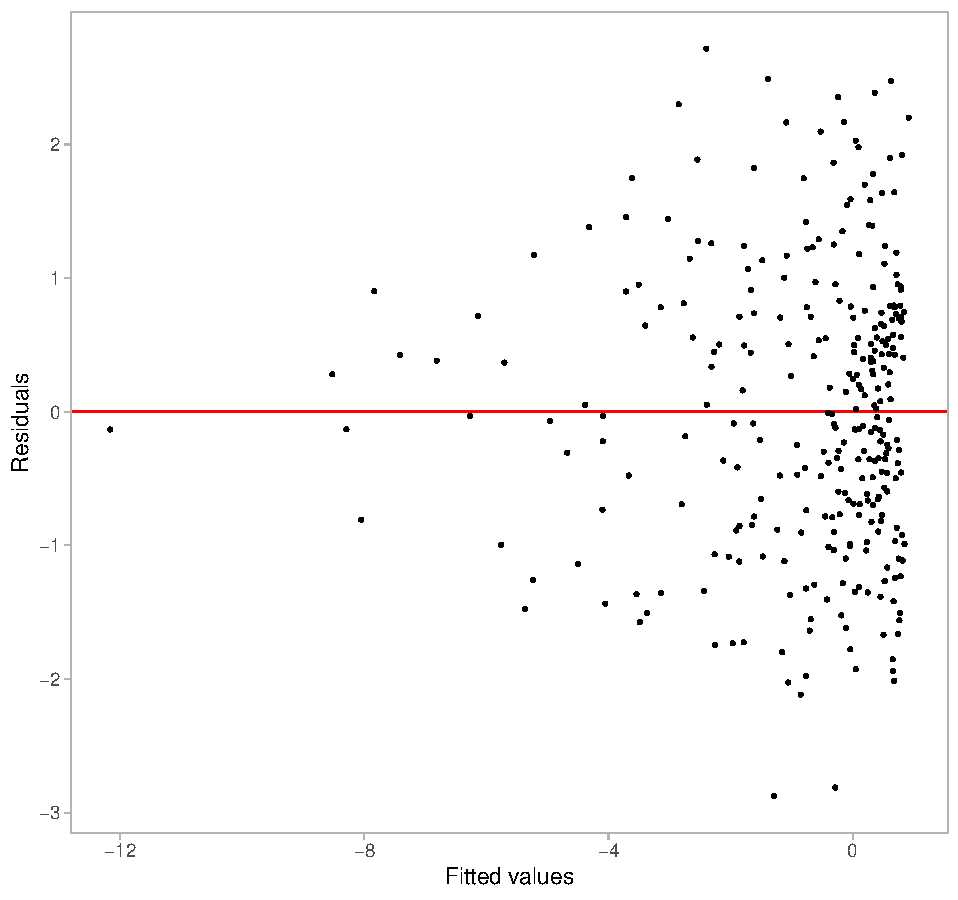
\includegraphics[width=1\linewidth]{paper_files/figure-latex/false-finding-1} 

}

\caption{An example residual vs fitted values plot (red line indicates 0). The vertical spread of the data points varies with the fitted values. This often indicates the existence of heteroskedasticity.}\label{fig:false-finding}
\end{figure}

\hypertarget{methodology}{%
\section{Methodology}\label{methodology}}

\hypertarget{different-possible-configurations-of-the-model-formula}{%
\subsection{Different possible configurations of the model
formula}\label{different-possible-configurations-of-the-model-formula}}

In addressing a problem, there exist multiple avenues for solutions.
Various configurations of the computer vision model formula can
effectively read residual plots, and these configurations can be
categorized based on two key components of the model formula: the input
and the output format.

\hypertarget{different-input-formats}{%
\subsubsection{Different input formats}\label{different-input-formats}}

In computer vision models, the input plays a role similar to predictors
in a linear regression model. The quality and relevance of the input
data greatly influence the model's capacity to generate insightful and
meaningful results. A straightforward approach involves feeding the
model a vector of residuals along with a vector of fitted values,
essentially providing all the necessary details for creating a residuals
vs fitted values plot. However, a drawback of this method is the dynamic
input size, as different fitted regression models may have varying
numbers of observations. In modern computer vision models created with
mainstream software like TensorFlow (ref here), the input is typically a
fixed-shape tensor. One solution is to pad the input vector with leading
or trailing zeros if the input tensor expects a longer vector. However,
this approach may fail if the input vector surpasses the designed
length. Another strategy is to summarize the residuals and fitted values
separately using histograms and utilize the counts as the input. By
controlling the number of bins in the histograms, it becomes possible to
provide a fixed-length input vector.

The primary advantage of using an image as input, as opposed to a vector
input format, relates to the development of sophisticated image
processing architectures over the years (see ref here). These
architectures effectively capture and summarize spatial information from
nearby pixels, which is less straightforward with vector input. The only
considerations are the image resolution and the aesthetics of the
residual plot. In general, higher resolution provides more information
to the model but comes with the trade-off of increased complexity and
greater difficulty in training. As for the aesthetics of the residual
plot, a practical solution is to consistently present residual plots in
the same style to the model. This implies that the model can not accept
arbitrary images as input but requires the use of the same preprocessing
software to convert provided residuals and fitted values into a
standardized style for the residual plot.

Other possible input formats include, but are not limited to, a pair of
residual plots, a triplet, and a lineup. Existing computer vision models
designed for image comparison can assess whether a pair of images are
similar or dissimilar (as seen in LeCun's 2005 paper). Applied to our
specific problem, we can define null plots of a fitted model to be
similar to each other, while considering actual residual plots to be
distinct from null plots of any fitted model. A triplet constitutes a
set of three images, denoted as \(image_1\), \(image_2\) and
\(image_3\). In computer vision models, triplets are often used to
predict whether \(image_2\) or \(image_3\) is more similar to
\(image_1\), proving particularly useful for establishing rankings
between samples. In the context of our problem, we can apply the same
criteria to define similarity between images. However, it's important to
note that these two approaches usually require additional considerations
regarding the loss function and, at times, non-standard training
processes due to shared weights between different convolutional blocks.

Presenting a lineup to a model and asking it to predict which residual
plot is the most different one aligns closely with the lineup protocol.
However, if the lineup consists of around 20 plots, similar to previous
human subject experiments (reference here), the resolution of the input
image could become quite large, posing challenges in training the model.
In fact, we experimented with this approach in a pilot study, and the
model's performance was sub-optimal.

We did not explore all the mentioned input formats due to the
considerable costs associated with data preparation and model training.
Considering the implementation cost and the interpretability of the
model, we settled on the single residual plot input format.

\hypertarget{different-output-formats}{%
\subsubsection{Different output
formats}\label{different-output-formats}}

Given that the input is a single residual plot represented as a
fixed-resolution image, the computer vision model's output can take one
of two formats: binary or numeric. This choice determines whether the
model is a classification model or a regression model. The binary
outcome might indicates whether the input image is a null plot or not,
or whether the input image would be rejected in a visual test conducted
by humans. The latter option requires data from prior human subject
experiments, posing challenges in controlling the quality and quantity
of data due to variations in experimental settings across different
studies. Additionally, some visual inference experiments are unrelated
to linear regression models and residual plots, resulting in a limited
amount of available training data.

Alternatively, the output could be a meaningful numeric measure, such as
the average distance to good residual plots. This approach necessitates
defining a distance measure between residual plots, which may be a
non-trivial task. However, once a meaningful distance measure is
established, the computer vision model's prediction becomes an
interpretable value with tangible significance. Studies have
demonstrated that defining a proper distance between images can enhance
the matching accuracy in image search compared to a binary outcome model
(ref here).

The following section will propose the distance measure used for
training the computer vision model.

\hypertarget{distance-from-the-good-residual-plots}{%
\subsection{Distance from the good residual
plots}\label{distance-from-the-good-residual-plots}}

In a visual test, the observer will be asked to choose one or more plots
that stand out as most distinct from others in a given lineup. To
develop a computer vision model for evaluating residual plots within the
visual inference framework, it is important to precisely define a
numerical measure of ``difference'' or ``distance'' between plots. This
distance can take the form of a basic statistical operation on pixels,
such as the sum of square differences. Alternatively, it could involve
established image similarity metrics like the Structural Similarity
Index Measure \citep{wang2004image}. The challenge lies in the fact that
metrics tailored for image comparison may not be suitable for evaluating
data plots, where only essential plot elements require assessment
\citep{chowdhury2018measuring}. Furthermore, scagnostics mentioned in
Section \ref{introduction} could be used to construct distance metrics
for data plots comparison, but the functional form still needs to be
carefully refined to accurately reflect the extent of the violations.

\hypertarget{residual-distribution}{%
\subsubsection{Residual distribution}\label{residual-distribution}}

The distance metrics proposed in this paper takes into account the fact
that we try to measure how different a residual plot is from a good
residual plot, or in other words, how different a given fitted model is
from a correctly specified model. For the classical normal linear
regression model, residuals are derived from the fitted values
\(\hat{\boldsymbol{y}}\) and observed values \(\boldsymbol{y}\). Suppose
the data generating process is known and the model is correctly
specified, by the Frisch-Waugh-Lowell theorem \citep{frisch1933partial},
residuals \(\boldsymbol{e}\) can also be written as a linear
transformation of the error \(\boldsymbol{\varepsilon}\) formulated as
\(\boldsymbol{e} = \boldsymbol{R}\boldsymbol{\varepsilon}\), where
\(\boldsymbol{R}=\boldsymbol{I}_n -\boldsymbol{X}(\boldsymbol{X}'\boldsymbol{X})^{-1}\boldsymbol{X}'\)
is the residual operator, \(\boldsymbol{X}\) is the design matrix,
\(\boldsymbol{I}_n\) is a \(n\) by \(n\) identity matrix, and \(n\) is
the number of observations.

One of the assumptions of the classical normal linear regression model
is the error \(\boldsymbol{\varepsilon}\) follows a multivariate normal
distribution with zero mean and constant variance, i.e.,
\(\boldsymbol{\varepsilon} \sim N(\boldsymbol{0}_n,\sigma^2\boldsymbol{I}_n)\).
It can be known that residuals \(\boldsymbol{e}\) also follow a certain
probability distribution transformed from the multivariate normal
distribution, which will be denoted as \(Q\). This reference
distribution \(Q\) summarizes what good residuals should follow given
the predictors are known and fixed.

When fitting a linear regression model, the solver will force
\(\sum_{i=1}^{n} e_i = 0\), making any residual value to be a linear
combination of the remaining \(n - 1\) residuals. This effectively means
\(rank(\boldsymbol{R}) = n - 1 < n\) and \(Q\) becomes a degenerate
multivariate distribution. To capture the characteristics of \(Q\), such
as moments, we can simulate a large numbers of
\(\boldsymbol{\varepsilon}\) and transform it to \(\boldsymbol{e}\) to
get the empirical estimates. For simplicity, we replaced
\(\boldsymbol{R}\) with a full-rank diagonal matrix
\(diag(\boldsymbol{R})\), where \(diag(.)\) set the non-diagonal entries
of a matrix to zeros. The resulting distribution for \(\boldsymbol{Q}\)
is \(N(\boldsymbol{0}_n, diag(\boldsymbol{R}\sigma^2))\).

Distribution \(Q\) is derived from the correctly specified model.
However, if the model is misspecified, then the actual distribution of
residuals denoted as \(P\), will be different to \(Q\). For example, if
the data generating process contains variables correlated with any
column of \(\boldsymbol{X}\) but not included in \(\boldsymbol{X}\),
causing an omitted variable problem, \(P\) will be different to \(Q\)
because the residual operator obtained from the fitted model will not be
the same as \(\boldsymbol{R}\). Besides, if the
\(\boldsymbol{\varepsilon}\) follows a non-normal distribution such as a
multivariate lognormal distribution, the empirical residual distribution
will usually be skewed and has a long tail.

\hypertarget{kullback-leibler-divergence-of-p-from-q}{%
\subsubsection{\texorpdfstring{Kullback-Leibler divergence of \(P\) from
\(Q\)}{Kullback-Leibler divergence of P from Q}}\label{kullback-leibler-divergence-of-p-from-q}}

Define a proper distance between distributions is usually easier than
define a proper distance between data plots. Given the actual residual
distribution \(Q\) and the reference residual distribution \(P\), we
used a distance metric based on Kullback-Leibler divergence
\citep{kullback1951information} to quantify the difference between two
distributions

\begin{align}
\label{eq:kl-0}
D &= log\left(1 + KL\right), \\
\label{eq:kl-1}
KL &= \int_{\mathbb{R}^{n}}log\frac{p(\boldsymbol{e})}{q(\boldsymbol{e})}p(\boldsymbol{e})d\boldsymbol{e},
\end{align}

\noindent where \(p(.)\) is the probability density function for
distribution \(P\), and \(q(.)\) is the probability density function for
distribution \(Q\).

This distance metric was first proposed in \citet{li2023plot}. It was
mainly designed for measuring the effect size of non-linearity and
heteroskedasticity in a residual plot. \citet{li2023plot} showed that,
for a classical normal linear regression model that omits a necessary
higher-order predictors \(\boldsymbol{Z}\), and incorrectly assumes
\(\boldsymbol{\varepsilon} \sim N(\boldsymbol{0}_n,\sigma^2\boldsymbol{I}_n)\)
while in fact
\(\boldsymbol{\varepsilon} \sim N(\boldsymbol{0}_n, \boldsymbol{V})\),
\(Q\) can be represented as
\(N(\boldsymbol{R}\boldsymbol{Z}\boldsymbol{\beta}_z, diag(\boldsymbol{R}\boldsymbol{V}\boldsymbol{R}'))\).
Note that the variance-covariance matrix is replaced with the diagonal
matrix to ensure it is a full-rank matrix.

Since both \(P\) and \(Q\) are adjusted to be multivariate normal
distributions, equation \ref{eq:kl-1} can be further expanded to

\begin{align}
\label{eq:kl-2}
KL &= \frac{1}{2}\left(\log\frac{|\text{diag}(\boldsymbol{W})|}{|\text{diag}(\boldsymbol{R}\sigma^2)|} - n + \text{tr}(\text{diag}(\boldsymbol{W})^{-1}\text{diag}(\boldsymbol{R}\sigma^2)) + \boldsymbol{\mu}_z'(diag(\boldsymbol{W}))^{-1}\boldsymbol{\mu}_z\right),
\end{align}

\noindent where
\(\boldsymbol{\mu}_z = \boldsymbol{R}\boldsymbol{Z}\boldsymbol{\beta}_z\),
and \(\boldsymbol{W} = \boldsymbol{R}\boldsymbol{V}\boldsymbol{R}'\).
The assumed error variance \(\sigma^2\) is set to be
\(tr(\boldsymbol{V})/n\), which is the expectation of the estimated
variance.

\hypertarget{evaluation-of-kullback-leibler-divergence-for-non-normal-p}{%
\subsubsection{\texorpdfstring{Evaluation of Kullback-Leibler divergence
for non-normal
\(P\)}{Evaluation of Kullback-Leibler divergence for non-normal P}}\label{evaluation-of-kullback-leibler-divergence-for-non-normal-p}}

For non-normal error \(\boldsymbol{\varepsilon}\), the actual residual
distribution \(P\) is unlikely to be a multivariate normal distribution.
Thus, equation \ref{eq:kl-2} given in \citet{li2023plot} will not be
applicable to models with non-normality violations.

To evaluate the Kullback-Leibler divergence of non-normal \(P\) from
\(Q\), the fallback is to solve equation \ref{eq:kl-1} numerically.
However, since \(\boldsymbol{e}\) is a linear transformation of
non-normal random variables, it is very common that the general form of
\(P\) is unknown, meaning that we can not easily compute
\(p(\boldsymbol{e})\) using a well-known probability density function.
Additionally, even if \(p(\boldsymbol{e})\) can be calculated for any
\(\boldsymbol{e} \in \mathbb{R}^n\), it will be very difficult to do
numerical integration over the \(n\) dimensional space, because \(n\)
could be potentially very large.

In order to evaluate equation \ref{eq:kl-1} in a practically computable
manner, the elements of \(\boldsymbol{e}\) are assumed to be independent
of each other. This assumption solves both of the issues mentioned
above. First, we no longer need to integrate over \(n\) random
variables. The result of equation \ref{eq:kl-1} is now the sum of the
Kullback-Leibler divergence evaluated for each individual residual
thanks for the independence assumption. Second, it is not required to
know the joint probability density \(p(\boldsymbol{e})\) any more.
Instead, the evaluation of Kullback-Leibler divergence for an individual
residual relies on the knowledge of the marginal density \(p_i(e_i)\),
where \(e_i\) is the \(i\)-th residual for \(i = 1, ..., n\). This is
much easier to estimate through simulation.

The algorithm for computing equation \ref{eq:kl-1} starts from
simulating \(m\) sets of \(\boldsymbol{\varepsilon}\) according to the
error distribution. The simulated errors are stored in a matrix
\(\boldsymbol{A}\) with \(n\) rows and \(m\) columns. So each column of
\(\boldsymbol{A}\) is a set of realization values of
\(\boldsymbol{\varepsilon}\). Then, we can get \(m\) sets of
\(\boldsymbol{e}\) stored in the matrix \(\boldsymbol{B}\) by applying
the residual operator \(\boldsymbol{B} = \boldsymbol{R}\boldsymbol{A}\).
Furthermore, kernel density estimation (KDE) with Gaussian kernel and
optimal bandwidth selected by the Silverman's rule of thumb
\citep{silverman2018density} is applied on each row of \(B\) to estimate
\(p_i(e_i)\) for \(i = 1, ..., n\). The KDE computation is done by the
\texttt{density} function in R.

Since the Kullback-Leibler divergence can be viewed as the expectation
of the log-likelihood ratio between distribution \(P\) and distribution
\(Q\) evaluated on distribution \(P\), we can reuse the simulated
residuals in matrix \(\boldsymbol{B}\) to estimate the expectation by
the sample mean. With the independence assumption, for non-normal \(P\),
\(KL\) can be estimated by

\begin{align}
\label{eq:kl-3}
\hat{KL} &= \sum_{i = 1}^{n} \hat{KL_i}, \\
\hat{KL_i} &= \frac{1}{m}\sum_{j = 1}^{m} log\frac{\hat{p_i}(B_{ij})}{q(B_{ij})},
\end{align}

\noindent where \(\hat{KL_i}\) is the estimator of the Kullback-Leibler
divergence for an individual residual \(e_i\), \(B_{ij}\) is the
\(i\)-th row and \(j\)-th column entry of the matrix \(B\),
\(\hat{p_i}(.)\) is the kernel density estimator of \(p_i(.)\), \(q(.)\)
is the normal density function with mean zero and an assumed variance
estimated as
\(\hat{\sigma^2} = \sum_{b \in vec(B)}(b - \sum_{b \in vec(B)} b/nm)^2/(nm - 1)\),
and \(vec(.)\) is the vectorization operator which turns a
\(n \times m\) matrix into a \(nm \times 1\) column vector by stacking
the columns of the matrix on top of each other.

\hypertarget{approximation-of-the-distance-metric}{%
\subsubsection{Approximation of the distance
metric}\label{approximation-of-the-distance-metric}}

In the previous sections, we have defined a distance metric given in
equation \ref{eq:kl-0} for quantifying the difference between the actual
residual distribution \(P\) and an ideal reference distribution \(Q\).
You may have noticed that this distance metric can only be computed when
the data generating process is known. In reality, we often have no
knowledge about the data generating process, otherwise we do not need to
fit a linear regression model in the first place.

What we proposed in this paper is a method to approximate this distance
with a residual plot. Let \(D\) be the result of equation \ref{eq:kl-0}
indicating the extent of the model violations, and our estimator
\(\hat{D}\) is formulated as

\begin{equation}
\label{eq:d-approx}
\hat{D} = cv(plot_{h\times w}(\boldsymbol{e}, \hat{\boldsymbol{y}})),
\end{equation}

\noindent where \(\boldsymbol{e}\) is a vector of residuals obtained
from the fitted model rather than a vector of random variables,
\(\hat{\boldsymbol{y}}\) is the fitted values also obtained from the
fitted model, \(plot(.)_{h \times w}\) is a plotting function that
generates a residuals vs fitted values plot with fixed aesthetic and
then saves it as an image with \(h \times w\) pixels and three colour
channels, and \(cv(.)\) is a computer vision model which takes an
\(h \times w\) image as input and predicts the distance in the domain
\([0, +\infty)\).

With the approximated distance \(\hat{D}\), we will be able to know how
different the underlying distribution of the residuals is from a good
residual distribution. This is meaningful way to check if a residual
plot is a good residual plot, and to know the strength of the visual
signal embedded in the residual plot.

The approximated distance \(\hat{D}\) is not expected to be the same as
the original distance \(D\). This is largely because information
contained in a single residual plot is limited and it may not be able to
summarise all the characteristics of the residual distribution. For a
given residual distribution \(P\), we can generate many different
residual plots. Some of them share similar visual patterns, but some of
them could be visually very different from the rest, especially for
models with small \(n\). This suggests the error of the approximation
will vary depends on whether the observed residual plot is
representative or not.

\hypertarget{statistical-testing-based-on-the-approximated-distance}{%
\subsection{Statistical testing based on the approximated
distance}\label{statistical-testing-based-on-the-approximated-distance}}

\hypertarget{null-distribution-of-the-approximated-distance}{%
\subsubsection{Null distribution of the approximated
distance}\label{null-distribution-of-the-approximated-distance}}

Having a computer vision model \(cv\) which gives an approximated
distance between \(0\) and \(+\infty\) is not enough to determine if the
null hypothesis that the model is correctly specified should be
rejected. Theoretically, the distance \(D\) for a correctly specified
model is \(0\), because \(P\) will be the same as \(Q\), and
\(log(1 + 0) = 0\). The computer vision model may not necessary predict
\(0\) for a null plot. Using \ref{fig:false-finding} as an example, it
contains a visual pattern which is an indication of heteroskedasticity.
We would not expect the model to be able to magically tell if the
suspicious pattern is caused by the skewed distribution of the fitted
values or the existence of heteroskedasticity. Assume we only train the
model with this single image, while \(50\)\% of the time the label is
\(0\), and \(50\)\% of the time the label is some constant greater than
\(0\). Then, a perfect model will predict a value between \(0\) and that
constant to achieve a minimum loss. So, it is expected that our computer
vision models will also predict value greater than \(0\) for some null
plots. It will make more sense if we interpret the model prediction as
the visual signal strength of the residual plot. Some null plots could
have outliers or strong visual patterns due to randomness, and the model
will try to summarise those information into the prediction.

To align with the principle of visual inference, we need to provide a
valid null distribution for the test statistic. If we treat the
approximated distance \(\hat{D}\) as a test statistic, then the null
distribution of this statistic can be approximated by the empirical
distribution of \(\hat{D}\) for a large amount of null plots of given a
fitted model. The procedure involves applying the residual rotation
technique \citep{buja2009statistical} on the fitted model to obtain null
residuals. The null residuals are then used to make null plots and fed
into the model. The results are used to construct an empirical
distribution.

\hypertarget{estimation-of-quantiles-of-the-null-distribution}{%
\subsubsection{Estimation of quantiles of the null
distribution}\label{estimation-of-quantiles-of-the-null-distribution}}

With the null distribution of the test statistic,

\begin{itemize}
\tightlist
\item
  How many null samples are needed to get stable 95\% quantile
\item
  How do we make decision based on the quantile (reject or not reject)
\item
  p-value calculation (percentage of null vss \textgreater{} vss)
\end{itemize}

\hypertarget{bootstrapping-the-approximated-distance}{%
\subsubsection{Bootstrapping the approximated
distance}\label{bootstrapping-the-approximated-distance}}

\begin{itemize}
\tightlist
\item
  What is the assumption of bootstrapping
\item
  Any drawback: loss of information
\item
  For each bootstrapped fitted model, we can get a bootstrapped vss and
  construct a new 95\% quantile for the null distribution, and check if
  H\_0 should be rejected
\item
  However, it is very expensive to construct a new 95\% quantile for
  each bootstrapped fitted model
\item
  The 95\% quantile constructed using the original fitted model can be
  considered as an estimate of those new 95\% quantiles
\item
  We borrow information from the original fitted model
\item
  We can check how many bootstrapped fitted model should be rejected
  (like the percentage)
\item
  This gives an overall estimate of how often the assumed regression
  model are considered to be incorrect if the data can be obtained
  repetitively from the same data generating process
\item
  If this percentage is relatively large, it gives the analyst an
  warning that the regression model is inappropriate to the data
\end{itemize}

\hypertarget{generation-of-training-data}{%
\subsection{Generation of training
data}\label{generation-of-training-data}}

\hypertarget{data-generating-process}{%
\subsubsection{Data generating process}\label{data-generating-process}}

While observational data is frequently employed in training models for
real-world applications, the data generating process of observational
data often remains unknown, making computation for our target variable
\(D\) unattainable. Consequently, the computer vision models developed
in this study were trained using synthetic data. This approach provides
us with precise label annotations. Additionally, it ensures a large and
diverse training dataset, as we have control over the data generating
process, and the simulation of the training data is relatively
cost-effective.

We have incorporated three types of residual departures of linear
regression model in the training data, including non-linearity,
heteroskedasticity and non-normality. All three departures can be
summarised by the data generating process formulated as

\begin{align}
\label{eq:data-sim}
\boldsymbol{y} &= \boldsymbol{1}_n + \boldsymbol{x}_1 + \beta_1\boldsymbol{x}_2 + \beta_2(\boldsymbol{z} + \beta_1\boldsymbol{w}) + \boldsymbol{k} \odot \boldsymbol{\varepsilon}, \\
\boldsymbol{z} &= He_j(g(\boldsymbol{x}_1, 2)), \\
\boldsymbol{w} &= He_j(g(\boldsymbol{x}_2, 2)), \\
\boldsymbol{k} &= \sqrt{\boldsymbol{1}_n + b(2 - |a|)(\boldsymbol{x}_1 + \beta_1\boldsymbol{x}_2 - a\boldsymbol{1}_n)^2},
\end{align}

\noindent where \(\boldsymbol{y}\), \(\boldsymbol{x}_1\),
\(\boldsymbol{x}_2\), \(\boldsymbol{z}\), \(\boldsymbol{w}\),
\(\boldsymbol{k}\) and \(\boldsymbol{\varepsilon}\) are vectors of size
\(n\), \(\boldsymbol{1}_n\) is a vector of ones of size \(n\),
\(\boldsymbol{x}_1\) and \(\boldsymbol{x}_2\) are two independent
predictors, \(He_j(.)\) is the \(j\)th-order probabilist's Hermite
polynomials \citep{hermite1864nouveau}, the \(\sqrt{(.)}\) and \((.)^2\)
operators are element-wise operators, \(\odot\) is the Hadamard product,
and \(g(., k)\) is a scaling function to enforce the support of the
random vector to be \([-k, k]^n\) defined as

\[g(\boldsymbol{x}, k) = 2k \cdot \frac{\boldsymbol{x} - x_{min}\boldsymbol{1}_n}{x_{max} - x_{min}} - k\boldsymbol{1}_n,~for~k > 0,\]
\noindent where \(x_{min} = \underset{i \in \{ 1,...,n\}}{min} x_i\),
\(x_{max} = \underset{i \in \{ 1,...,n\}}{max} x_i\) and \(x_i\) is the
\(i\)-th entry of \(\boldsymbol{x}\).

The residuals and fitted values of the fitted model is obtained by
regressing \(\boldsymbol{y}\) on \(\boldsymbol{x}_1\). This data
generating process is adopted from \citet{li2023plot} where it was used
to simulate residual plots with non-linearity and heteroskedasticity
visual patterns for human subject experiments.

In equation \ref{eq:data-sim}, predictor \(\boldsymbol{x}_1\) and
\(\boldsymbol{x}_2\) are independent of each other, so excluding
\(\boldsymbol{x}_2\) from the regression formula will not cause any
problem. However, \(\boldsymbol{z}\) and \(\boldsymbol{w}\) are
higher-order terms of \(\boldsymbol{x}_1\) and \(\boldsymbol{x}_2\). If
\(\beta_2 \neq 0\), the regression model will suffer from non-linearity
issues. Parameter \(j\) is a shape parameter controlling the number of
tuning points of the non-linearity pattern. Generally, greater values of
\(j\) will result in more tuning points.

Additionally, Scaling factor \(\boldsymbol{k}\) directly affects the
error distribution and it is correlated with \(\boldsymbol{x}_1\) and
\(\boldsymbol{x}_2\). If \(b \neq 0\) and
\(\boldsymbol{\varepsilon} \sim N(\boldsymbol{0}_n, \sigma^2\boldsymbol{I}_n)\),
the constant variance assumption will be violated. Parameter \(a\) is a
shape parameter controlling the location of the smallest variance in a
residual plot.

Non-normality violations are introduced by defining a non-normal
distribution for \(\boldsymbol{\varepsilon}\).

\begin{itemize}
\tightlist
\item
  distribution of x1 and x2
\item
  summary table of all the factor values
\item
  example plots for the violations
\end{itemize}

\hypertarget{computation-of-scagnostics}{%
\subsubsection{Computation of
scagnostics}\label{computation-of-scagnostics}}

We have mentioned in Section \ref{introduction} that scagnostics
summarise some useful characteristics of the scatter plot. Although the
computer vision model will learn the feature extraction function during
the training process, it will be beneficial to utilize scagnostics to
help computer vision model making more accurate predictions as these
measure could provide additional useful information.

For each generated residual plot, four scagnostics, namely,
``Monotonic'', ``Sparse'', ``Splines'' and ``Striped'' are computed
using the \texttt{cassowaryr} R package (ref here). The computed
measures along with the number of observations of the fitted model are
provided as the second input of the computer vision model.

Other scagnostics are also informative, but unfortunately, they are
unavailable due to a fatal bug in the compiled C program of the
\texttt{interp} R package (ref here) that will crash the process in a
unpredictable manner. For reproducibility, we do not include these
scagnostics in the training data.

\hypertarget{crafting-a-balanced-training-set}{%
\subsubsection{Crafting a balanced training
set}\label{crafting-a-balanced-training-set}}

In order to train a robust computer vision model, we intentionally
control the distribution of the target variable \(D\) of the training
data. Making it uniform between \(0\) and \(7\). This is accomplished by
preparing \(50\) buckets each only accepts training samples with \(D\)
between \([7(i - 1)/49, 7i/49)\) for \(i < 50\), where \(i\) is the
index of the \(i\)-th bucket. For the \(50\)-th bucket, any training
samples with \(D >= 7\) will be accepted. We have prepared 80000
training images, so each bucket can only contain
\(80000 \div 50 = 1600\) training samples. The simulator will repeatedly
sample parameter values from the parameter sample, generate residuals
and fitted values using the data generating process, compute the
distance, and check if the sample can be accepted by the corresponding
bucket, until all the buckets are full.

\hypertarget{architecture-of-the-computer-vision-model}{%
\subsection{Architecture of the computer vision
model}\label{architecture-of-the-computer-vision-model}}

\begin{itemize}
\tightlist
\item
  optimization (MSE loss function, with equation)
\item
  a diagram
\item
  explain the existence of removable layers
\item
  explain three different resolutions
\end{itemize}

\hypertarget{training-process-and-hyperparameter-tuning}{%
\subsection{Training process and hyperparameter
tuning}\label{training-process-and-hyperparameter-tuning}}

\begin{itemize}
\tightlist
\item
  software environment (tf and keras)
\item
  tuner (keras\_tuner)
\item
  80\% validation data, 20\% training data
\item
  100 trials (Bayesian optimizer)
\item
  monitor RMSE
\item
  early stopping (50 epochs)
\item
  learning rate reduction (10 epochs, 0.5 factor)
\item
  max 2000 epochs (no one reach)
\item
  restore best epoch of the best trial
\end{itemize}

\hypertarget{model-evaluation-methods}{%
\subsection{Model evaluation methods}\label{model-evaluation-methods}}

\begin{itemize}
\tightlist
\item
  RMSE for the test set
\item
  R\^{}2
\item
  Mean bias deviation to understand the overall bias
\item
  quantile loss to understand how well the model captures the entire
  distribution of D
\item
  Percentage of predictions within a tolerance interval (like 0.1)
\end{itemize}

\hypertarget{results}{%
\section{Results}\label{results}}

\hypertarget{best-model-performance}{%
\subsection{Best model performance}\label{best-model-performance}}

\begin{itemize}
\tightlist
\item
  Metrics for model performance
\item
  Shap values
\item
  Heatmap
\end{itemize}

\hypertarget{comparison-with-human-visual-inference}{%
\subsection{Comparison with human visual
inference}\label{comparison-with-human-visual-inference}}

\hypertarget{overview-of-the-human-subject-experiment}{%
\subsubsection{Overview of the human subject
experiment}\label{overview-of-the-human-subject-experiment}}

\hypertarget{comparison}{%
\subsubsection{Comparison}\label{comparison}}

\begin{itemize}
\tightlist
\item
  power comparison
\item
  decisions
\end{itemize}

\hypertarget{when-the-model-works}{%
\subsection{When the model works}\label{when-the-model-works}}

\begin{itemize}
\tightlist
\item
  simple examples (non-linearity, heteroskedasticity, \ldots)
\item
  datasaurus
\end{itemize}

\hypertarget{when-the-model-does-not-work}{%
\subsection{When the model does not
work}\label{when-the-model-does-not-work}}

\begin{itemize}
\tightlist
\item
  human detect but model does not
\item
  cartoon residuals?
\end{itemize}

\hypertarget{workflow-how-one-use-this-model-small-showcase}{%
\subsection{Workflow: how one use this model? (small
showcase)}\label{workflow-how-one-use-this-model-small-showcase}}

\hypertarget{dicussion}{%
\section{Dicussion}\label{dicussion}}

There are other kinds of residual departures like autocorrelation that
are not considered in this study. The primary goal of this paper is to
establish a new way of evaluating residual plot and conducting visual
test with computer vision models. Building computer vision models for
other model violations and other types of diagnostic plots could be
future directions of this field.

\hypertarget{conclusion}{%
\section{Conclusion}\label{conclusion}}

\begin{itemize}
\tightlist
\item
  Summary of findings
\item
  Contributions to the field
\item
  Future directions for research
\end{itemize}

\bibliographystyle{tfcad}
\bibliography{ref.bib}





\end{document}
